\documentclass[aspectratio=169]{beamer}
\usepackage{xcolor}
\usepackage{tikz}
\usetikzlibrary{patterns}
\usepackage{amsmath, amssymb, bm, amsfonts}
\usepackage{multicol}
\usetikzlibrary{tikzmark}
\usepackage[table]{xcolor}
\usepackage{array}

% settings for the beamer theme
\usetheme[progressbar= frametitle]{metropolis}
%\setbeamertemplate{frame numbering}[fraction]
\setbeamertemplate{footline}{}
\useoutertheme{metropolis}
\useinnertheme{metropolis}
\usecolortheme{spruce}
\setbeamercolor{background canvas}{bg=white}
\definecolor{mygreen}{rgb}{.125, .5, .125}
\usecolortheme[named=mygreen]{structure}

% setting for the title
%\title[Short Title]{Beamer-Krumel}
\title{\Huge Teoría de Conjuntos}
%\subtitle{Subtitle Here}
\usepackage{graphicx} % Required for inserting images
\author{\textbf{\Large Kenyer Aguiar}}
%\institute{Institute}
\institute{\large\textbf{Objetivo de la clase:} \\[6pt]
Practicar ejercicios de Teoría de Conjuntos.}
\date{}

% No tocar permite que align y \pause funcionen bien
\mode<presentation> { \setbeamercovered{transparent=0} }
\makeatletter
\def\pdftex@driver{pdftex.def}
\ifx\Gin@driver\pdftex@driver
  \def\pgfsys@color@unstacked#1{%
    \pdfliteral{\csname\string\color@#1\endcsname}%
  }
\fi
\makeatother
%------------------------------



% Definir color gris claro
\definecolor{grisclaro}{RGB}{235,235,235}

% Entorno personalizado sin título
\newenvironment{mibloque}
{
\begin{center}
\begin{beamercolorbox}[
    rounded=true,
    shadow=false,
    sep=1em,
    wd=0.8\textwidth
]{}
\setbeamercolor{background canvas}{bg=grisclaro}
\color{black}
\setbeamercolor{block body}{bg=grisclaro}
\begin{beamercolorbox}[rounded=false,sep=0.3em,wd=\textwidth]{block body}
}
{
\end{beamercolorbox}
\end{beamercolorbox}
\end{center}
}

%------------------------------


\newcommand{\cuadro}[1]{
\tikz[baseline=(m.base)]{
        \node[draw=mygreen, text=mygreen, inner sep=2pt, thick, anchor=base, fill = mygreen!10] (m) {#1}
        ;}\quad}



\newcommand{\ejemplo}{%
  \tikz[baseline=(m.base)]{
    \node[
      draw=mygreen,
      text=mygreen,
      inner sep=2pt,
      thick,
      anchor=base,
      fill=mygreen!10
    ] (m) {\textbf{Ejemplo}};
  }%
\,\,}

\newcommand{\sol}{%
  \tikz[baseline=(m.base)]{
    \node[
      draw=mygreen,
      text=mygreen,
      inner sep=2pt,
      thick,
      anchor=base,
      fill=mygreen!10
    ] (m) {\textbf{Solución:}};
  }%
\,\,}
        
\begin{document}
% filling for blocks
\metroset{block=fill}

\begin{frame}
	\titlepage
\end{frame}


\begin{frame}[t]{}
	\Large
	\begin{block}{Ejercicio 8}
		Si los conjuntos $A$ y $B$ son iguales, donde
		\[
			A=\{3a+5,\,7\}, \qquad B=\left\{\frac{b}{2}-3,\,5\right\},
		\]
		determine el valor de $a-b$.
	\end{block}
\end{frame}

\begin{frame}[t]{}
	\begin{block}{Ejercicio 10}
		\Large
		Sea $
			P=\{3,\{7\},\{9,10\},\{4\},2,4\}.$
		Indique si las siguientes afirmaciones son verdaderas (V) o falsas (F), según corresponda:
		\begin{multicols}{2}
			\begin{enumerate}[A)]
				\item $2 \in P$
				\item  $\{2\} \subset P$
				\item $\{9,10\} \subset P$
				\item $\{\{4\}\} \subset P$
				\item $\varnothing \subset P$
				\item $0\in P$
			\end{enumerate}
		\end{multicols}
	\end{block}
\end{frame}

\begin{frame}[t]{}
	\begin{block}{Ejercicio 11}
		Si $A=\{7, 8, 5 ,4 ,3\}$,  B=\{5 , 4, 9, 10\} y  $C=\{4, 9, 7, 12\}$ y el conjunto universo es $U=\{x\in\mathbb{N}: 1\leq x\leq 15\}.$
		Hallar
		\begin{multicols}{3}
			\begin{enumerate}
				\item $A\cup B$
				\item $A\cup C$
				\item $B\cap C$
				\item $A\cup B\cup C$
				\item $ (A \cup B)\cap C$
				\item $A-B$
				\item $B-C$
				\item $A-(B\cup C)$
				\item $A\cap B\cap C$
				\item $A^c$
				\item $B^c$
				\item $C^c$
				\item $(A\cup B)^c$
				\item $A^c \cap B^c$
				\item $(C\cap B)^c\cap A^c
				      $
			\end{enumerate}
		\end{multicols}
	\end{block}
\end{frame}


\begin{frame}[t]{}

	\begin{block}{Ejercicio 13}
		\Large
		Sean los conjuntos
		\[
			A=\{1,3,5,7,9,12\}, \qquad B=\{3,9,8,10,11\}.
		\]

		Entonces, indique si las siguientes afirmaciones son verdaderas (V) o falsas (F):
		\begin{multicols}{2}
			\begin{enumerate}
				\item $8\in A\cap B$
				\item $12\in (A\cap B)$
				\item $\#(A\cup B)=11$
				\item $(A\cup B)-(A\cap B)=\{1,5,7,8,10,11\}$
			\end{enumerate}
		\end{multicols}
	\end{block}
\end{frame}

\begin{frame}[t]{}
	\begin{block}{Ejercicio 26}
		\Large
		Los siguientes conjuntos son unitarios e iguales
		$A = \{2a+b, c\}$;
		$B = \{2c -7, 5b+2\}$.
		Calcule a +b+c.
	\end{block}
\end{frame}

\begin{frame}[t]{Lanzamiento de dos dados}
	\begin{block}{Ejercicio 1}
		En un lanzamiento de dos dados, se define el conjunto $A$ como el conjunto de los resultados posibles del dado número 1, y el conjunto $B$ como el conjunto de los resultados posibles del dado número 2.

		\begin{enumerate}
			\item Determine por extensión los conjuntos $A$ y $B$.
			\item Determine por extensión el conjunto $A\times B$.
		\end{enumerate}
	\end{block}
\end{frame}



\begin{frame}[t]{Lanzamiento de dados}
	\begin{block}{Ejercicio 2}
		Sean $A$, $B$ los conjuntos definidos en el ejercicio anterior.Represente gráficamente el conjunto $A\times B$.
	\end{block}\pause
	\begin{center}
		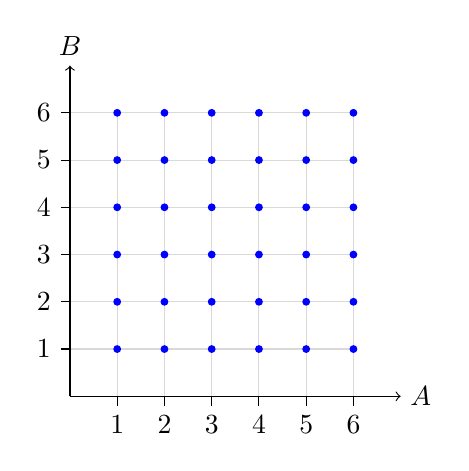
\begin{tikzpicture}[scale=0.6]
			% Ejes
			% Cuadrícula opcional
			\draw[step=1cm, gray!30, thin] (0,0) grid (6,6);
			\draw[->] (0,0) -- (7,0) node[right] {$A$};
			\draw[->] (0,0) -- (0,7) node[above] {$B$};

			% Marcas eje X
			\foreach \x in {1,...,6}
				{
					\draw (\x,0) -- (\x,-0.2) node[below] {\x};
				}

			% Marcas eje Y
			\foreach \y in {1,...,6}
				{
					\draw (0,\y) -- (-0.2,\y) node[left] {\y};
				}

			% Puntos del producto cartesiano
			\foreach \x in {1,...,6}
				{
					\foreach \y in {1,...,6}
						{
							\filldraw[blue] (\x,\y) circle (2pt);
						}
				}


		\end{tikzpicture}
	\end{center}


\end{frame}

\begin{frame}[t]
	\frametitle{Lanzamiento de dados}
	\begin{block}{Ejercicio 3}
		Sea $C=\{(a, b)\in A\times B: a+b=7\}$. Hallar $C$ por extensión, resente gráficamente el conjunto $C$ y determine su cardinalidad.
	\end{block}


	\renewcommand{\arraystretch}{1.3} % altura de filas
	\begin{flushleft}
		\begin{tabular}{|c|*{6}{c|}}
			\hline
			\cellcolor{gray!30} \textbf{+}
			                                & \cellcolor{yellow} \textbf{1}
			                                & \cellcolor{yellow} \textbf{2}
			                                & \cellcolor{yellow} \textbf{3}
			                                & \cellcolor{yellow} \textbf{4}
			                                & \cellcolor{yellow} \textbf{5}
			                                & \cellcolor{yellow} \textbf{6}               \\
			\hline
			\cellcolor{green!70} \textbf{1} &                               &  &  &  &  & \\ \hline
			\cellcolor{green!70} \textbf{2} &                               &  &  &  &  & \\ \hline
			\cellcolor{green!70} \textbf{3} &                               &  &  &  &  & \\ \hline
			\cellcolor{green!70} \textbf{4} &                               &  &  &  &  & \\ \hline
			\cellcolor{green!70} \textbf{5} &                               &  &  &  &  & \\ \hline
			\cellcolor{green!70} \textbf{6} &                               &  &  &  &  & \\
			\hline
		\end{tabular}
	\end{flushleft}



\end{frame}
\begin{frame}[t]
	\frametitle{Lanzamiento de dados}
	\begin{block}{Ejercicio 4}
		Sea $D=\{(a, b)\in A\times B: a+b>5\}$. Hallar $D$ por extensión, resente gráficamente el conjunto $D$ y determine su cardinalidad.
	\end{block}


	\renewcommand{\arraystretch}{1.3} % altura de filas
	\begin{flushleft}
		\begin{tabular}{|c|*{6}{c|}}
			\hline
			\cellcolor{gray!30} \textbf{+}
			                                & \cellcolor{yellow} \textbf{1}
			                                & \cellcolor{yellow} \textbf{2}
			                                & \cellcolor{yellow} \textbf{3}
			                                & \cellcolor{yellow} \textbf{4}
			                                & \cellcolor{yellow} \textbf{5}
			                                & \cellcolor{yellow} \textbf{6}               \\
			\hline
			\cellcolor{green!70} \textbf{1} &                               &  &  &  &  & \\ \hline
			\cellcolor{green!70} \textbf{2} &                               &  &  &  &  & \\ \hline
			\cellcolor{green!70} \textbf{3} &                               &  &  &  &  & \\ \hline
			\cellcolor{green!70} \textbf{4} &                               &  &  &  &  & \\ \hline
			\cellcolor{green!70} \textbf{5} &                               &  &  &  &  & \\ \hline
			\cellcolor{green!70} \textbf{6} &                               &  &  &  &  & \\
			\hline
		\end{tabular}
	\end{flushleft}



\end{frame}

\begin{frame}[t]
	\frametitle{Lanzamiento de dados}
	\begin{block}{Ejercicio 5}
		Sea $E=\{(a, b)\in A\times B: a+b\leq 10\}$. Hallar $E$ por extensión, resente gráficamente el conjunto $E$ y determine su cardinalidad.
	\end{block}


	\renewcommand{\arraystretch}{1.3} % altura de filas
	\begin{flushleft}
		\begin{tabular}{|c|*{6}{c|}}
			\hline
			\cellcolor{gray!30} \textbf{+}
			                                & \cellcolor{yellow} \textbf{1}
			                                & \cellcolor{yellow} \textbf{2}
			                                & \cellcolor{yellow} \textbf{3}
			                                & \cellcolor{yellow} \textbf{4}
			                                & \cellcolor{yellow} \textbf{5}
			                                & \cellcolor{yellow} \textbf{6}               \\
			\hline
			\cellcolor{green!70} \textbf{1} &                               &  &  &  &  & \\ \hline
			\cellcolor{green!70} \textbf{2} &                               &  &  &  &  & \\ \hline
			\cellcolor{green!70} \textbf{3} &                               &  &  &  &  & \\ \hline
			\cellcolor{green!70} \textbf{4} &                               &  &  &  &  & \\ \hline
			\cellcolor{green!70} \textbf{5} &                               &  &  &  &  & \\ \hline
			\cellcolor{green!70} \textbf{6} &                               &  &  &  &  & \\
			\hline
		\end{tabular}
	\end{flushleft}
\end{frame}

\begin{frame}[t]
	\frametitle{Lanzamiento de dados}
	\begin{block}{Ejercicio 6}
		Sea $F=\{(a, b)\in A\times B: a+b\text{ es par}\}$. Hallar $F$ por extensión, resente gráficamente el conjunto $F $ y determine su cardinalidad.
	\end{block}


	\renewcommand{\arraystretch}{1.3} % altura de filas
	\begin{flushleft}
		\begin{tabular}{|c|*{6}{c|}}
			\hline
			\cellcolor{gray!30} \textbf{+}
			                                & \cellcolor{yellow} \textbf{1}
			                                & \cellcolor{yellow} \textbf{2}
			                                & \cellcolor{yellow} \textbf{3}
			                                & \cellcolor{yellow} \textbf{4}
			                                & \cellcolor{yellow} \textbf{5}
			                                & \cellcolor{yellow} \textbf{6}               \\
			\hline
			\cellcolor{green!70} \textbf{1} &                               &  &  &  &  & \\ \hline
			\cellcolor{green!70} \textbf{2} &                               &  &  &  &  & \\ \hline
			\cellcolor{green!70} \textbf{3} &                               &  &  &  &  & \\ \hline
			\cellcolor{green!70} \textbf{4} &                               &  &  &  &  & \\ \hline
			\cellcolor{green!70} \textbf{5} &                               &  &  &  &  & \\ \hline
			\cellcolor{green!70} \textbf{6} &                               &  &  &  &  & \\
			\hline
		\end{tabular}
	\end{flushleft}
\end{frame}

\begin{frame}[t]
	\frametitle{Lanzamiento de dados}
	\begin{block}{Ejercicio 7}
		Sea $G=\{(a, b)\in A\times B: a+b=1\}$. Hallar $G$ por extensión, resente gráficamente el conjunto $G $ y determine su cardinalidad.
	\end{block}


	\renewcommand{\arraystretch}{1.3} % altura de filas
	\begin{flushleft}
		\begin{tabular}{|c|*{6}{c|}}
			\hline
			\cellcolor{gray!30} \textbf{+}
			                                & \cellcolor{yellow} \textbf{1}
			                                & \cellcolor{yellow} \textbf{2}
			                                & \cellcolor{yellow} \textbf{3}
			                                & \cellcolor{yellow} \textbf{4}
			                                & \cellcolor{yellow} \textbf{5}
			                                & \cellcolor{yellow} \textbf{6}               \\
			\hline
			\cellcolor{green!70} \textbf{1} &                               &  &  &  &  & \\ \hline
			\cellcolor{green!70} \textbf{2} &                               &  &  &  &  & \\ \hline
			\cellcolor{green!70} \textbf{3} &                               &  &  &  &  & \\ \hline
			\cellcolor{green!70} \textbf{4} &                               &  &  &  &  & \\ \hline
			\cellcolor{green!70} \textbf{5} &                               &  &  &  &  & \\ \hline
			\cellcolor{green!70} \textbf{6} &                               &  &  &  &  & \\
			\hline
		\end{tabular}
	\end{flushleft}
\end{frame}


\begin{frame}[t]
	\frametitle{Lanzamiento de dados}
	\begin{block}{Ejercicio 8}
		Sea $H=\{(a, b)\in A\times B: a+b\text{ es cuadrado perfecto}\}$. Hallar $H$ por extensión, resente gráficamente el conjunto $H $ y determine su cardinalidad.
	\end{block}


	\renewcommand{\arraystretch}{1.3} % altura de filas
	\begin{flushleft}
		\begin{tabular}{|c|*{6}{c|}}
			\hline
			\cellcolor{gray!30} \textbf{+}
			                                & \cellcolor{yellow} \textbf{1}
			                                & \cellcolor{yellow} \textbf{2}
			                                & \cellcolor{yellow} \textbf{3}
			                                & \cellcolor{yellow} \textbf{4}
			                                & \cellcolor{yellow} \textbf{5}
			                                & \cellcolor{yellow} \textbf{6}               \\
			\hline
			\cellcolor{green!70} \textbf{1} &                               &  &  &  &  & \\ \hline
			\cellcolor{green!70} \textbf{2} &                               &  &  &  &  & \\ \hline
			\cellcolor{green!70} \textbf{3} &                               &  &  &  &  & \\ \hline
			\cellcolor{green!70} \textbf{4} &                               &  &  &  &  & \\ \hline
			\cellcolor{green!70} \textbf{5} &                               &  &  &  &  & \\ \hline
			\cellcolor{green!70} \textbf{6} &                               &  &  &  &  & \\
			\hline
		\end{tabular}
	\end{flushleft}
\end{frame}


\begin{frame}[t]{Pregunta de análisis}
	En el lanzamiento de dos dados, cuál es la probabilidad de que los dados sumen 7 en un lanzamiento?. Si tuvieras que apostar, ¿apostarías a que los dados sumen 7? Justifica tu respuesta.
\end{frame}

\end{document}